% This LaTeX document needs to be compiled with XeLaTeX.
\documentclass[10pt]{article}
\usepackage[utf8]{inputenc}
\usepackage{amsmath}
\usepackage{amsfonts}
\usepackage{amssymb}
\usepackage[version=4]{mhchem}
\usepackage{stmaryrd}
\usepackage{graphicx}
\usepackage[export]{adjustbox}
\graphicspath{ {./images/} }
\usepackage{hyperref}
\hypersetup{colorlinks=true, linkcolor=blue, filecolor=magenta, urlcolor=cyan,}
\urlstyle{same}
\usepackage{multirow}
\usepackage[fallback]{xeCJK}
\usepackage{polyglossia}
\usepackage{fontspec}
\setCJKmainfont{Noto Serif CJK TC}

\setmainlanguage{polish}
\setmainfont{CMU Serif}

\author{Czas pracy 170 minut}
\date{}


\begin{document}
\maketitle
\section*{PRÓBNY EGZAMIN MATURALNY Z MATEMATYKI}
\section*{POZIOM PODSTAWOWY}


\section*{Instrukcja dla piszącego}
\begin{enumerate}
  \item Sprawdź, czy arkusz zawiera 16 stron.
  \item W zadaniach od 1. do 20. są podane 4 odpowiedzi: A, B, C, D, z których tylko jedna jest prawdziwa. Wybierz tylko jedna odpowiedź i zaznacz ją na karcie odpowiedzi.
  \item Zaznaczając odpowiedzi w części karty przeznaczonej dla zdającego, zamaluj \(\square\) pola do tego przeznaczone. Błędne zaznaczenie otocz kółkiem i zaznacz właściwe.
  \item Rozwiązania zadań od 21. do 30. zapisz starannie i czytelnie w wyznaczonych miejscach. Przedstaw swój tok rozumowania prowadzący do ostatecznego wyniku.
  \item Pisz czytelnie. Używaj długopisu/pióra tylko z czarnym tuszem/atramentem.
  \item Nie używaj korektora. Błędne zapisy przekreśl.
  \item Pamiętaj, że zapisy w brudnopisie nie podlegają ocenie.
  \item Obok numeru każdego zadania jest podana maksymalna liczba punktów możliwych do uzyskania.
  \item Możesz korzystać z zestawu wzorów matematycznych, cyrkla i linijki oraz kalkulatora.
  \item Wypełnij tę część karty odpowiedzi, którą koduje zdający. Nie wpisuj żadnych znaków w częşci przeznaczonej dla egzaminatora.
\end{enumerate}

Życzymy powodzenia!

MARZEC\\
ROK 2012

Za rozwiązanie wszystkich zadań można otrzymać łącznie do\\
50 punktów

Wypelnia zdający przed\\
rozpoczęciem pracy\\
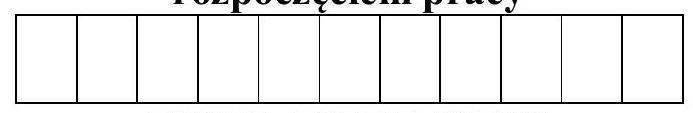
\includegraphics[max width=\textwidth, center]{2024_11_21_2c2c97b7feae6d70b078g-01}

PESEL ZDAJĄCEGO

Odpowiedzi z tej próbnej matury znajdziesz dziś o godzinie 14 na \href{http://www.echodnia.eu/edukacja}{www.echodnia.eu/edukacja} oraz w jutrzejszym wydaniu papierowym „Echa Dnia"

\section*{ZADANIA ZAMKNIETE}
\section*{W zadaniach od 1. do 20. wybierz jedna poprawna odpowiedz.}
\section*{Zadanie 1. (1 pkt)}
Wskaż nierówność, którą spełnia liczba \(5 \sqrt{3}\)\\
A. \(|x-1|<2\)\\
B. \(|x-2|<3\)\\
C. \(|x-3|<4\)\\
D. \(|x-4|<5\)

\section*{Zadanie 2. (1 pkt)}
Gdy \(a+b=10\), to wówczas wartość wyrażenia \(\frac{2 a^{2}+4 a b+2 b^{2}}{(a+b)^{3}}\) jest równa\\
A. 10\\
B. 100\\
C. \(\frac{1}{5}\)\\
D. \(\frac{1}{10}\)

\section*{Zadanie 3. (1 pkt)}
Cena kurtki po dwóch kolejnych obniżkach, za każdym razem o 10\% jest równa 202 zł 50 gr. Przed obniżkami cena tej kurtki była równa\\
A. \(202 \mathrm{zł} 70 \mathrm{gr}\)\\
B. \(222 \mathrm{zł} 50 \mathrm{gr}\)\\
C. 243 zt\\
D. 250 zl

\section*{Zadanie 4. (1 pkt)}
Liczba \(128^{-4}:\left(\frac{1}{32}\right)^{4}\) jest równa\\
A. \(4^{-4}\)\\
B. \(2^{-4}\)\\
C. \(2^{4}\)\\
D. \(4^{4}\)

\section*{Zadanie 5. (1 pkt)}
Liczba \(2 \log _{3} 27-\log _{2} 16\) jest równa\\
A. 2\\
B. -8\\
C. 9\\
D. \(\frac{3}{2}\)

Zadanie 6. (1 pkt)\\
Zbiorem wszystkich rozwiązań nierówności \(x \sqrt{3}+4 \geq 2 x+\sqrt{12}\) jest przedział\\
A. \((-\infty, 2)\)\\
B. \((-\infty, 2\rangle\)\\
C. \(\langle 2,+\infty)\)\\
D. \((2,+\infty)\)

Zadanie 7. (1 pkt)\\
Liczba wszystkich rozwiązań równania \((2 x-3)\left(x^{2}-x\right)=0\) jest równa\\
A. 0\\
B. 1\\
C. 2\\
D. 3

Zadanie 8. (1 pkt)\\
Miejscem zerowym funkcji liniowej \(f(x)=-2 x+m+7\) jest liczba 3. Wynika stąd, że\\
A. \(m=7\)\\
B. \(m=1\)\\
C. \(m=-1\)\\
D. \(m=-7\)

\section*{Zadanie 9. (1 pkt)}
Dla każdego \(x \neq 2\) wyrażenie \(\frac{x-1}{3 x-6}-\frac{2}{x-2}\) jest równe\\
A. \(\frac{x+1}{3 x-6}\)\\
B. \(\frac{x+5}{3 x-6}\)\\
C. \(\frac{x-7}{3 x-6}\)\\
D. \(\frac{x-3}{3 x-6}\)

\section*{BRUDNOPIS}
www, ectionthines\\

\includegraphics[max width=\textwidth, center]{2024_11_21_2c2c97b7feae6d70b078g-03}\\
CK\\
RADIO

\section*{Zadanie 10. (1 pkt)}
Liczby 12, 18, \(2 x+1\) są, w podanej kolejności, odpowiednio pierwszym, drugim i trzecim wyrazem ciągu geometrycznego. Wynika stąd, że\\
A. \(x=11 \frac{1}{2}\)\\
B. \(x=12\)\\
C. \(x=12 \frac{1}{2}\)\\
D. \(x=13\)

\section*{Zadanie 11. (1 pkt)}
W ciągu arytmetycznym \(\left(a_{n}\right)\) dane są \(a_{1}=2\) i \(a_{2}=4\). Suma dziesięciu początkowych wyrazów tego ciągu jest równa\\
A. 30\\
B. 110\\
C. 220\\
D. 2046

Zadanie 12. (1 pkt)\\
Kąt \(\alpha\) jest ostry i \(\sin \alpha=0,6\). Wówczas\\
A. \(\cos \alpha=0,8\) i \(\operatorname{tg} \alpha=0,4\)\\
B. \(\cos \alpha=0,4\) i \(\operatorname{tg} \alpha=1,5\)\\
C. \(\cos \alpha=0,8\) i \(\operatorname{tg} \alpha=0,75\)\\
D. \(\cos \alpha=0,4\) i \(\operatorname{tg} \alpha=0,75\)

\section*{Zadanie 13. (1 pkt)}
Proste o równaniach \(y=2 x-5\) i \(y=(3-m) x+4\) są równoległe. Wynika stąd, że\\
A. \(m=1\)\\
B. \(m=\frac{5}{2}\)\\
C. \(m=\frac{7}{2}\)\\
D. \(m=5\)

\section*{Zadanie 14. (1 pkt)}
Proste \(A D\) i \(B C\) są równoległe. Długości odcinków \(E D, D C\) oraz \(A B\) podane są na rysunku. Długość odcinka \(E A\) jest równa\\
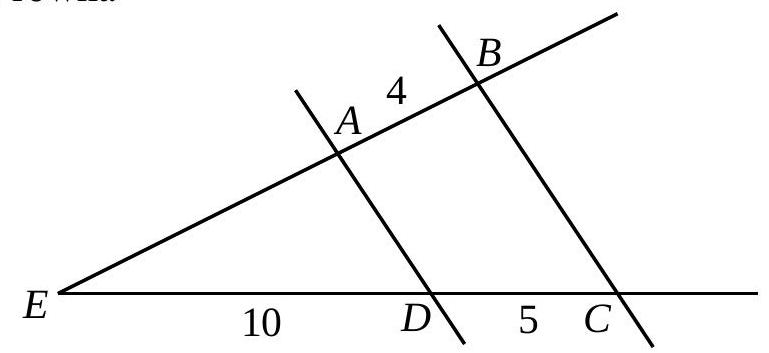
\includegraphics[max width=\textwidth, center]{2024_11_21_2c2c97b7feae6d70b078g-04}\\
A. 4\\
B. 8\\
C. 9\\
D. 10

\section*{Zadanie 15. (1 pkt)}
Rysunek przedstawia trapez prostokątny i długości trzech jego boków.\\
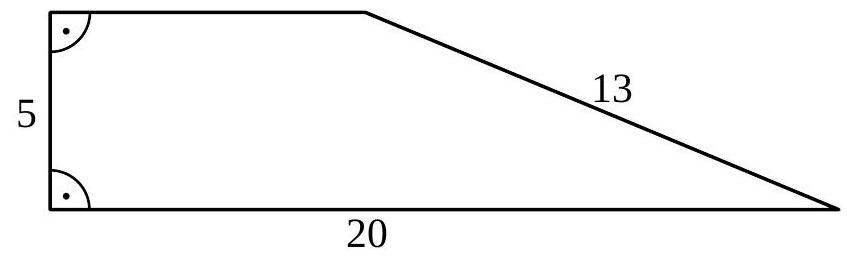
\includegraphics[max width=\textwidth, center]{2024_11_21_2c2c97b7feae6d70b078g-04(1)}

Obwód tego trapezu jest równy\\
A. 43\\
B. 46\\
C. 48\\
D. 50

Zadanie 16. (1 pkt)\\
Objętość sześcianu jest równa 27. Długość przekątnej tego sześcianu jest równa\\
A. \(2 \sqrt{2}\)\\
B. \(3 \sqrt{2}\)\\
C. \(2 \sqrt{3}\)\\
D. \(3 \sqrt{3}\)

\section*{BRUDNOPIS}
www.erchathes\\

\includegraphics[max width=\textwidth, center]{2024_11_21_2c2c97b7feae6d70b078g-05}\\
CK\\
RADIO

\section*{Zadanie 17. (1 pkt)}
Bok rombu ma długość 8 , a kąt ostry ma miarę \(60^{\circ}\). Wysokość tego rombu jest więc równa\\
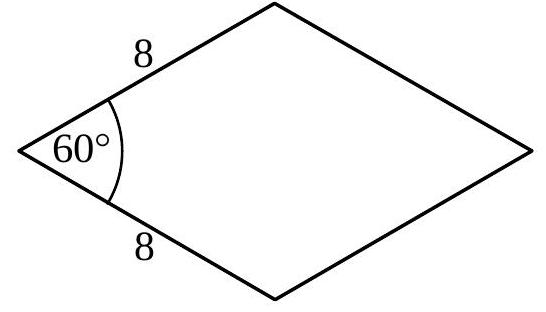
\includegraphics[max width=\textwidth, center]{2024_11_21_2c2c97b7feae6d70b078g-06(1)}\\
A. \(2 \sqrt{3}\)\\
B. \(4 \sqrt{3}\)\\
C. \(6 \sqrt{3}\)\\
D. \(8 \sqrt{3}\)

Zadanie 18. (1 pkt)\\
Punkty \(A, B, C, D\) i \(E\) leżą na okręgu o środku \(S\) i dzielą ten okrąg na pięć łuków równej długości (zobacz rysunek). Wówczas miara kąta ostrego \(\alpha\) między cięciwą \(A B\) i styczną do tego okręgu w punkcie \(A\) jest równa\\
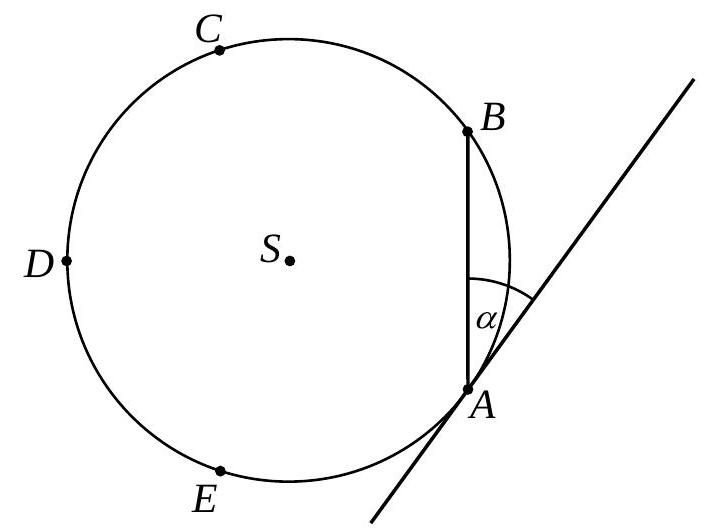
\includegraphics[max width=\textwidth, center]{2024_11_21_2c2c97b7feae6d70b078g-06}\\
A. \(\alpha=18^{\circ}\)\\
B. \(\alpha=30^{\circ}\)\\
C. \(\alpha=36^{\circ}\)\\
D. \(\alpha=54^{\circ}\)

\section*{Zadanie 19. (1 pkt)}
Tabela przedstawia zestawienie liczby błędów popełnionych przez zdających część teoretyczną egzaminu na prawo jazdy.

\begin{center}
\begin{tabular}{|l|c|c|c|c|}
\hline
Liczba błędów & 0 & 1 & 2 & \(x\) \\
\hline
Liczba zdających & 8 & 4 & 10 & 8 \\
\hline
\end{tabular}
\end{center}

Średnia arytmetyczna liczby tych błędów popełnionych przez jednego zdającego jest równa 1,6. Wynika stąd, że\\
A. \(x=3\)\\
B. \(x=4\)\\
C. \(x=5\)\\
D. \(x=6\)

\section*{Zadanie 20. (1 pkt)}
O zdarzeniach \(A\) oraz \(B\) zawartych w \(\Omega\) wiadomo, że \(P(A)=\frac{5}{6}, P(B)=\frac{2}{3}\) i \(A \cup B\) jest zdarzeniem pewnym. Wtedy\\
A. \(P(A \cap B)=\frac{1}{2}\)\\
B. \(\quad P(A \cap B)=\frac{1}{3}\)\\
C. \(P(A \cap B)=\frac{1}{4}\)\\
D. \(P(A \cap B)=\frac{1}{6}\)

\section*{BRUDNOPIS}
\section*{Zadanie 21. (2 pkt)}
Rozwiąż nierówność \(-2 x^{2}+3 x+2 \leq 0\).

\begin{center}
\begin{tabular}{|c|c|c|c|c|c|c|c|c|c|c|c|c|c|c|c|c|c|c|c|c|c|c|c|c|c|c|c|c|c|c|c|}
\hline
 &  &  &  &  &  &  &  &  &  &  &  &  &  &  &  &  &  &  &  &  &  &  &  &  &  &  &  &  &  &  &  \\
\hline
 &  &  &  &  &  &  &  &  &  &  &  &  &  &  &  &  &  &  &  &  &  &  &  &  &  &  &  &  &  &  &  \\
\hline
 &  &  &  &  &  &  &  &  &  &  &  &  &  &  &  &  &  &  &  &  &  &  &  &  &  &  &  &  &  &  &  \\
\hline
 &  &  &  &  &  &  &  &  &  &  &  &  &  &  &  &  &  &  &  &  &  &  &  &  &  &  &  &  &  &  &  \\
\hline
 &  &  &  &  &  &  &  &  &  &  &  &  &  &  &  &  &  &  &  &  &  &  &  &  &  &  &  &  &  &  &  \\
\hline
 &  &  &  &  &  &  &  &  &  &  &  &  &  &  &  &  &  &  &  &  &  &  &  &  &  &  &  &  &  &  &  \\
\hline
 &  &  &  &  &  &  &  &  &  &  &  &  &  &  &  &  &  &  &  &  &  &  &  &  &  &  &  &  &  &  &  \\
\hline
 &  &  &  &  &  &  &  &  &  &  &  &  &  &  &  &  &  &  &  &  &  &  &  &  &  &  &  &  &  &  &  \\
\hline
 &  &  &  &  &  &  &  &  &  &  &  &  &  &  &  &  &  &  &  &  &  &  &  &  &  &  &  &  &  &  &  \\
\hline
 &  &  &  &  &  &  &  &  &  &  &  &  &  &  &  &  &  &  &  &  &  &  &  &  &  &  &  &  &  &  &  \\
\hline
 &  &  &  &  &  &  &  &  &  &  &  &  &  &  &  &  &  &  &  &  &  &  &  &  &  &  &  &  &  &  &  \\
\hline
 &  &  &  &  &  &  &  &  &  &  &  &  &  &  &  &  &  &  &  &  &  &  &  &  &  &  &  &  &  &  &  \\
\hline
 &  &  &  &  &  &  &  &  &  &  &  &  &  &  &  &  &  &  &  &  &  &  &  &  &  &  &  &  &  &  &  \\
\hline
 &  &  &  &  &  &  &  &  &  &  &  &  &  &  &  &  &  &  &  &  &  &  &  &  &  &  &  &  &  &  &  \\
\hline
 &  &  &  &  &  &  &  &  &  &  &  &  &  &  &  &  &  &  &  &  &  &  &  &  &  &  &  &  &  &  &  \\
\hline
 & - &  &  &  &  &  &  &  &  &  &  &  &  &  &  &  &  &  &  &  &  &  &  &  &  &  &  &  &  &  &  \\
\hline
 &  &  &  &  &  &  &  &  &  &  &  &  &  &  &  &  &  &  &  &  &  &  &  &  &  &  &  &  &  &  &  \\
\hline
 & - &  &  &  &  &  &  &  &  &  &  &  &  &  &  &  &  &  &  &  &  &  &  &  &  &  &  &  &  &  &  \\
\hline
 &  &  &  &  &  &  &  &  &  &  &  &  &  &  &  &  &  &  &  &  &  &  &  &  &  &  &  &  &  &  &  \\
\hline
 &  &  &  &  &  &  &  &  &  &  &  &  &  &  &  &  &  &  &  &  &  &  &  &  &  &  &  &  &  &  &  \\
\hline
\end{tabular}
\end{center}

Odpowiedź:

\section*{Zadanie 22. (2 pkt)}
Oblicz największą wartość funkcji kwadratowej \(f(x)=-2 x^{2}+16 x-15\) w przedziale \(\langle-2,3\rangle\).\\
\(\qquad\)\\
Odpowiedź: \(\qquad\)

Zadanie 23. (2 pkt)\\
Powierzchnia boczna stożka po rozwinięciu na płaszczyznę jest ćwiartką koła o promieniu 8 cm . Oblicz wysokość tego stożka.\\

\includegraphics[max width=\textwidth, center]{2024_11_21_2c2c97b7feae6d70b078g-09(1)}

Odpowiedź:

\section*{Zadanie 24. (2 pkt)}
Ciąg \(\left(a_{n}\right)\) jest określony dla \(n \geq 1\) wzorem \(a_{n}=-n^{2}-4 \sqrt{3}\). Sprawdź, którym wyrazem tego ciągu jest liczba \(-3^{2}-(2+\sqrt{3})^{2}\).

\begin{center}
\begin{tabular}{|c|c|c|c|c|c|c|c|c|c|c|c|c|c|c|c|c|c|c|c|c|c|c|c|c|c|c|c|c|c|c|c|}
\hline
 &  &  &  &  &  &  &  &  &  &  &  &  &  &  &  &  &  &  &  &  &  &  &  &  &  &  &  &  &  &  &  \\
\hline
 &  &  &  &  &  &  &  &  &  &  &  &  &  &  &  &  &  &  &  &  &  &  &  &  &  &  &  &  &  &  &  \\
\hline
 &  &  &  &  &  &  &  &  &  &  &  &  &  &  &  &  &  &  &  &  &  &  &  &  &  &  &  &  &  &  &  \\
\hline
 &  &  &  &  &  &  &  &  &  &  &  &  &  &  &  &  &  &  &  &  &  &  &  &  &  &  &  &  &  &  &  \\
\hline
 &  &  &  &  &  &  &  &  &  &  &  &  &  &  &  &  &  &  &  &  &  &  &  &  &  &  &  &  &  &  &  \\
\hline
 &  &  &  &  &  &  &  &  &  &  &  &  &  &  &  &  &  &  &  &  &  &  &  &  &  &  &  &  &  &  &  \\
\hline
 &  &  &  &  &  &  &  &  &  &  &  &  &  &  &  &  &  &  &  &  &  &  &  &  &  &  &  &  &  &  &  \\
\hline
 &  &  &  &  &  &  &  &  &  &  &  &  &  &  &  &  &  &  &  &  &  &  &  &  &  &  &  &  &  &  &  \\
\hline
 &  &  &  &  &  &  &  &  &  &  &  &  &  &  &  &  &  &  &  &  &  &  &  &  &  &  &  &  &  &  &  \\
\hline
 &  &  &  &  &  &  &  &  &  &  &  &  &  &  &  &  &  &  &  &  &  &  &  &  &  &  &  &  &  &  &  \\
\hline
 &  &  &  &  &  &  &  &  &  &  &  &  &  &  &  &  &  &  &  &  &  &  &  &  &  &  &  &  &  &  &  \\
\hline
 &  &  &  &  &  &  &  &  &  &  &  &  &  &  &  &  &  &  &  &  &  &  &  &  &  &  &  &  &  &  &  \\
\hline
 &  &  &  &  &  &  &  &  &  &  &  &  &  &  &  &  &  &  &  &  &  &  &  &  &  &  &  &  &  &  &  \\
\hline
 &  &  &  &  &  &  &  &  &  &  &  &  &  &  &  &  &  &  &  &  &  &  &  &  &  &  &  &  &  &  &  \\
\hline
 & 
\includegraphics[max width=\textwidth]{2024_11_21_2c2c97b7feae6d70b078g-09}
 &  &  &  &  &  &  &  &  &  &  &  &  &  &  &  &  &  &  &  &  &  &  &  &  &  &  &  &  &  &  \\
\hline
 &  &  &  &  &  &  &  &  &  &  &  &  &  &  &  &  &  &  &  &  &  &  &  &  &  &  &  &  &  &  &  \\
\hline
 &  &  &  &  &  &  &  &  &  &  &  &  &  &  &  &  &  &  &  &  &  &  &  &  &  &  &  &  &  &  &  \\
\hline
 &  &  &  &  &  &  &  &  &  &  &  &  &  &  &  &  &  &  &  &  &  &  &  &  &  &  &  &  &  &  &  \\
\hline
\end{tabular}
\end{center}

Odpowiedź: \(\qquad\)

\section*{Zadanie 25. (2 pkt)}
Udowodnij, że dla dowolnych liczb rzeczywistych \(x, y, z\) takich, że \(x+y+z=3\) prawdziwa jest nierówność \(x^{2}+y^{2}+z^{2} \geq 3\).

\begin{center}
\begin{tabular}{|c|c|c|c|c|c|c|c|c|c|c|c|c|c|c|c|c|c|c|c|c|c|c|c|c|c|c|c|c|c|c|c|}
\hline
 &  &  &  &  &  &  &  &  &  &  &  &  &  &  &  &  &  &  &  &  &  &  &  &  &  &  &  &  &  &  &  \\
\hline
 &  &  &  &  &  &  &  &  &  &  &  &  &  &  &  &  &  &  &  &  &  &  &  &  &  &  &  &  &  &  &  \\
\hline
 &  &  &  &  &  &  &  &  &  &  &  &  &  &  &  &  &  &  &  &  &  &  &  &  &  &  &  &  &  &  &  \\
\hline
 &  &  &  &  &  &  &  &  &  &  &  &  &  &  &  &  &  &  &  &  &  &  &  &  &  &  &  &  &  &  &  \\
\hline
 &  &  &  &  &  &  &  &  &  &  &  &  &  &  &  &  &  &  &  &  &  &  &  &  &  &  &  &  &  &  &  \\
\hline
 &  &  &  &  &  &  &  &  &  &  &  &  &  &  &  &  &  &  &  &  &  &  &  &  &  &  &  &  &  &  &  \\
\hline
 &  &  &  &  &  &  &  &  &  &  &  &  &  &  &  &  &  &  &  &  &  &  &  &  &  &  &  &  &  &  &  \\
\hline
 &  &  &  &  &  &  &  &  &  &  &  &  &  &  &  &  &  &  &  &  &  &  &  &  &  &  &  &  &  &  &  \\
\hline
 &  &  &  &  &  &  &  &  &  &  &  &  &  &  &  &  &  &  &  &  &  &  &  &  &  &  &  &  &  &  &  \\
\hline
 &  &  &  &  &  &  &  &  &  &  &  &  &  &  &  &  &  &  &  &  &  &  &  &  &  &  &  &  &  &  &  \\
\hline
 &  &  &  &  &  &  &  &  &  &  &  &  &  &  &  &  &  &  &  &  &  &  &  &  &  &  &  &  &  &  &  \\
\hline
 &  &  &  &  &  &  &  &  &  &  &  &  &  &  &  &  &  &  &  &  &  &  &  &  &  &  &  &  &  &  &  \\
\hline
 &  &  &  &  &  &  &  &  &  &  &  &  &  &  &  &  &  &  &  &  &  &  &  &  &  &  &  &  &  &  &  \\
\hline
 &  &  &  &  &  &  &  &  &  &  &  &  &  &  &  &  &  &  &  &  &  &  &  &  &  &  &  &  &  &  &  \\
\hline
 &  &  &  &  &  &  &  &  &  &  &  &  &  &  &  &  &  &  &  &  &  &  &  &  &  &  &  &  &  &  &  \\
\hline
 &  &  &  &  &  &  &  &  &  &  &  &  &  &  &  &  &  &  &  &  &  &  &  &  &  &  &  &  &  &  &  \\
\hline
 &  &  &  &  &  &  &  &  &  &  &  &  &  &  &  &  &  &  &  &  &  &  &  &  &  &  &  &  &  &  &  \\
\hline
 &  &  &  &  &  &  &  &  &  &  &  &  &  &  &  &  &  &  &  &  &  &  &  &  &  &  &  &  &  &  &  \\
\hline
\end{tabular}
\end{center}

\section*{Zadanie 26. (2 pkt)}
Wykaż, że jeżeli ramiona \(A D\) i \(B C\) trapezu \(A B C D\) o podstawach \(A B\) i \(C D\) zawierają się w prostych prostopadłych (zobacz rysunek), to \(|A B|^{2}+|C D|^{2}=|A C|^{2}+|B D|^{2}\).\\
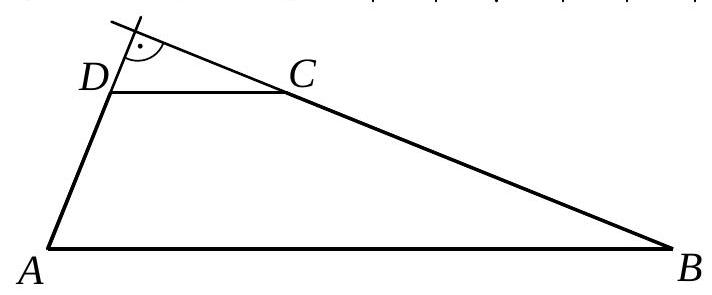
\includegraphics[max width=\textwidth, center]{2024_11_21_2c2c97b7feae6d70b078g-10}\\

\includegraphics[max width=\textwidth, center]{2024_11_21_2c2c97b7feae6d70b078g-10(1)}

Zadanie 27. (4 pkt)\\
Ze zbioru wszystkich liczb naturalnych czterocyfrowych losujemy jedną liczbę. Oblicz prawdopodobieństwo zdarzenia, że otrzymamy liczbę spełniającą jednocześnie trzy następujące warunki:\\
(1) liczba jest podzielna przez 25,\\
(2) cyfry dziesiątek i setek są nieparzyste,\\
(3) cyfra dziesiątek jest nie większa niż cyfra setek.\\

\includegraphics[max width=\textwidth, center]{2024_11_21_2c2c97b7feae6d70b078g-11}

Odpowiedź: \(\qquad\)

\section*{Zadanie 28. (5 pkt)}
Prostokątny pas wykładziny dywanowej o wymiarach \(3,6 \mathrm{~m}\) na \(7,5 \mathrm{~m}\) należy przeciąć prostopadle do dłuższego boku tak, aby przekątne otrzymanych dwóch prostokątnych kawałków różniły się o \(1,5 \mathrm{~m}\). Oblicz wymiary większego z otrzymanych kawałków.\\

\includegraphics[max width=\textwidth, center]{2024_11_21_2c2c97b7feae6d70b078g-12}

Odpowiedź: \(\qquad\)

\section*{Zadanie 29. (4 pkt)}
Prosta o równaniu \(y=x+2\) przecina okrąg o równaniu \((x-3)^{2}+(y-5)^{2}=25\) w punktach \(A\) i \(B\). Oblicz współrzędne punktów \(A\) i \(B\) oraz wyznacz równanie stycznej do danego okręgu przechodzącej przez jeden z tych punktów.\\

\includegraphics[max width=\textwidth, center]{2024_11_21_2c2c97b7feae6d70b078g-13}

Odpowiedź: \(\qquad\)

Zadanie 30. (5 pkt)\\
Podstawą ostrosłupa \(A B C D S\) jest kwadrat \(A B C D\). Wysokość SE ściany bocznej \(A D S\) jest jednocześnie wysokością ostrosłupa, a punkt \(E\) jest środkiem krawędzi \(A D\) (zobacz rysunek). Pole ściany \(A D S\) jest równe \(12 \mathrm{~cm}^{2}\), a objętość ostrosłupa jest równa \(48 \mathrm{~cm}^{3}\). Oblicz miarę kąta nachylenia krawędzi bocznej \(C S\) do płaszczyzny podstawy ostrosłupa. Wynik zaokrąglij do \(1^{\circ}\).\\
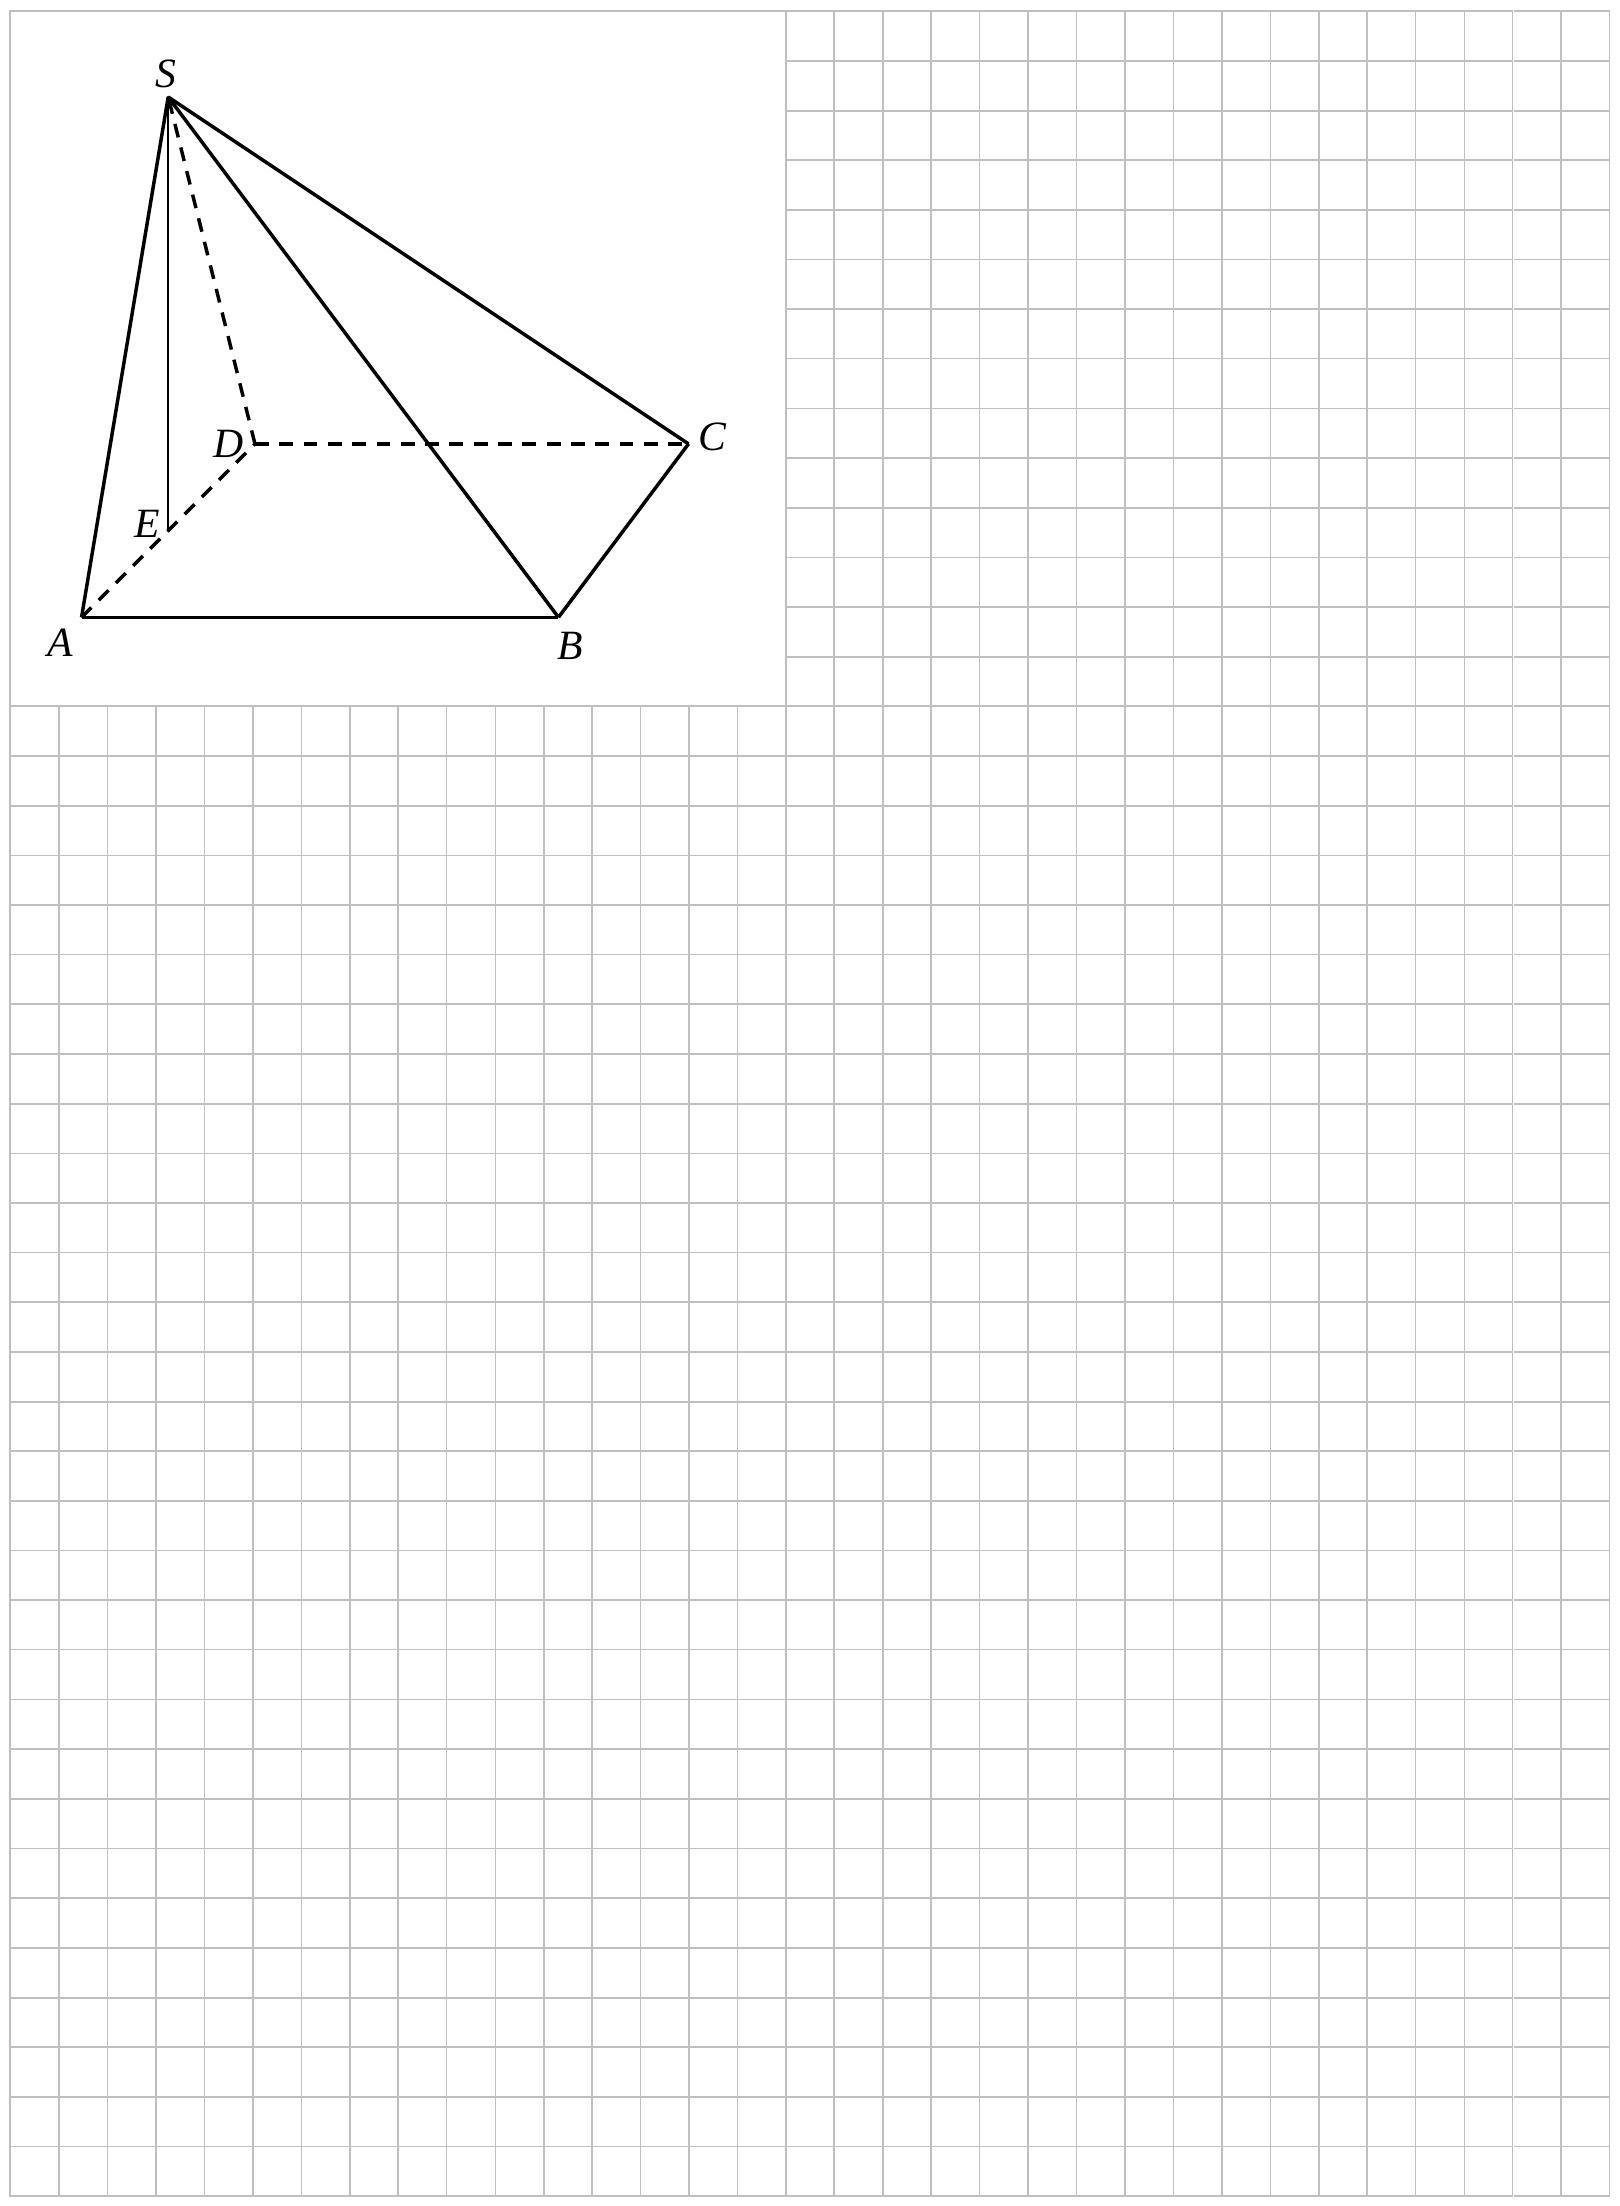
\includegraphics[max width=\textwidth, center]{2024_11_21_2c2c97b7feae6d70b078g-14}

Odpowiedź: \(\qquad\)

\section*{BRUDNOPIS}
\section*{KARTA ODPOWIEDZI}
PESEL\\
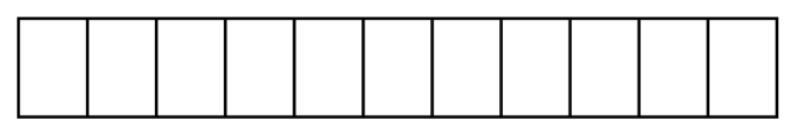
\includegraphics[max width=\textwidth, center]{2024_11_21_2c2c97b7feae6d70b078g-16(1)}

\begin{center}
\begin{tabular}{|c|c|c|c|c|}
\hline
 & \multicolumn{4}{|c|}{Odpowiedzi} \\
\hline
1 & 因 & B & C &  \\
\hline
2 & 因 & B & C & D \\
\hline
3 & 因 & B & C & D \\
\hline
4 & 因 & B & C & D \\
\hline
5 & 因 & B & C & D \\
\hline
6 & 因 & B & C & D \\
\hline
7 & 因 & B & C & D \\
\hline
8 & 因 & B & C &  \\
\hline
9 & 因 & B & C & ( \\
\hline
10 & 因 & B & C & D \\
\hline
11 & 因 & B & C & D \\
\hline
12 & 因 & B & C & D \\
\hline
13 & 因 & B & C & D \\
\hline
14 & 因 & B & C &  \\
\hline
15 & 因 & B & C & D \\
\hline
16 & 因 & B & C & D \\
\hline
17 & 因 & B & C & ■ \\
\hline
18 & 因 & B & C & ( \\
\hline
19 & 因 & B & C & D \\
\hline
20 & 因 & B & C & D \\
\hline
\end{tabular}
\end{center}

WYPEŁNIA EGZAMINATOR

\begin{center}
\begin{tabular}{|c|c|c|c|c|c|c|}
\hline
\multirow{2}{*}{\begin{tabular}{c}
Nr \\
zadania \\
\end{tabular}} & \multicolumn{6}{|c|}{Punkty} \\
\hline
 & \(\square\) & 1 & \(\square\) & \(\square\) &  &  \\
\hline
22 & \(\square\) & \(\square\) & \(\square\) &  &  &  \\
\hline
23 & \(\square\) & \(\square\) & \(\square\) &  &  &  \\
\hline
24 & \(\square\) & \(\square\) & \(\square\) &  &  &  \\
\hline
25 & \(\square\) & \(\square\) & \(\square\) &  &  &  \\
\hline
26 & \(\square\) & \(\square\) & \(\square\) &  &  &  \\
\hline
27 & \(\square\) & \(\square\) & \(\square\) & \(\square\) & \(\square\) &  \\
\hline
28 & \(\square\) & \(\square\) & \(\square\) & \(\square\) & \(\square\) & \(\square\) \\
\hline
29 & \(\square\) & \(\square\) & \(\square\) & \(\square\) & \(\square\) &  \\
\hline
30 & \(\square\) & \(\square\) & \(\square\) & \(\square\) & \(\square\) & \(\square\) \\
\hline
\end{tabular}
\end{center}

\begin{center}
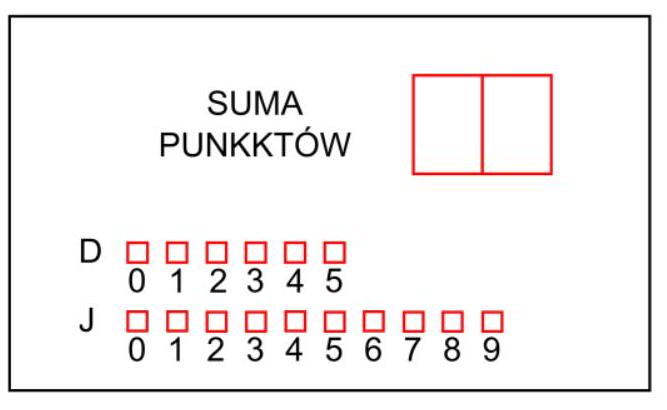
\includegraphics[max width=\textwidth]{2024_11_21_2c2c97b7feae6d70b078g-16}
\end{center}


\end{document}